\section{Experimental setup and measurement process}
\label{sec:Setup}
The apparatus to determine the heat capacity of copper can be seen in \autoref{fig:setup}.
The copper sample can be found in the recipient, which is located in the middle of a Dewar container. It is surrounded by a heating coil that can be used to
heat the sample while monitoring the input electric power. Another copper cylinder with a second heating coil is installed around the sample. This is needed to compensate the
black body radiation from the sample and prevent heat conduction.
The temperature of both copper pieces is measured using Pt-100 resistors connected to ohmmeters. Their resistance is a function of the temperature. The temperature in degrees Celsius can be calculated as
\begin{equation}
    \label{eqn:R_T}
    T(R) = \num{0.00134} R^2 + \num{2.296} R - \num{243.02}
\end{equation}
with the resistor's value $R$ in ohms.
A vacuum pump is used to evacuate the recipient. The apparatus can be cooled by filling liquid nitrogen in the Dewar container. During this process, helium is inserted into the recipient
through a helium bottle that is also connected to the apparatus.

\begin{figure}
    \centering
    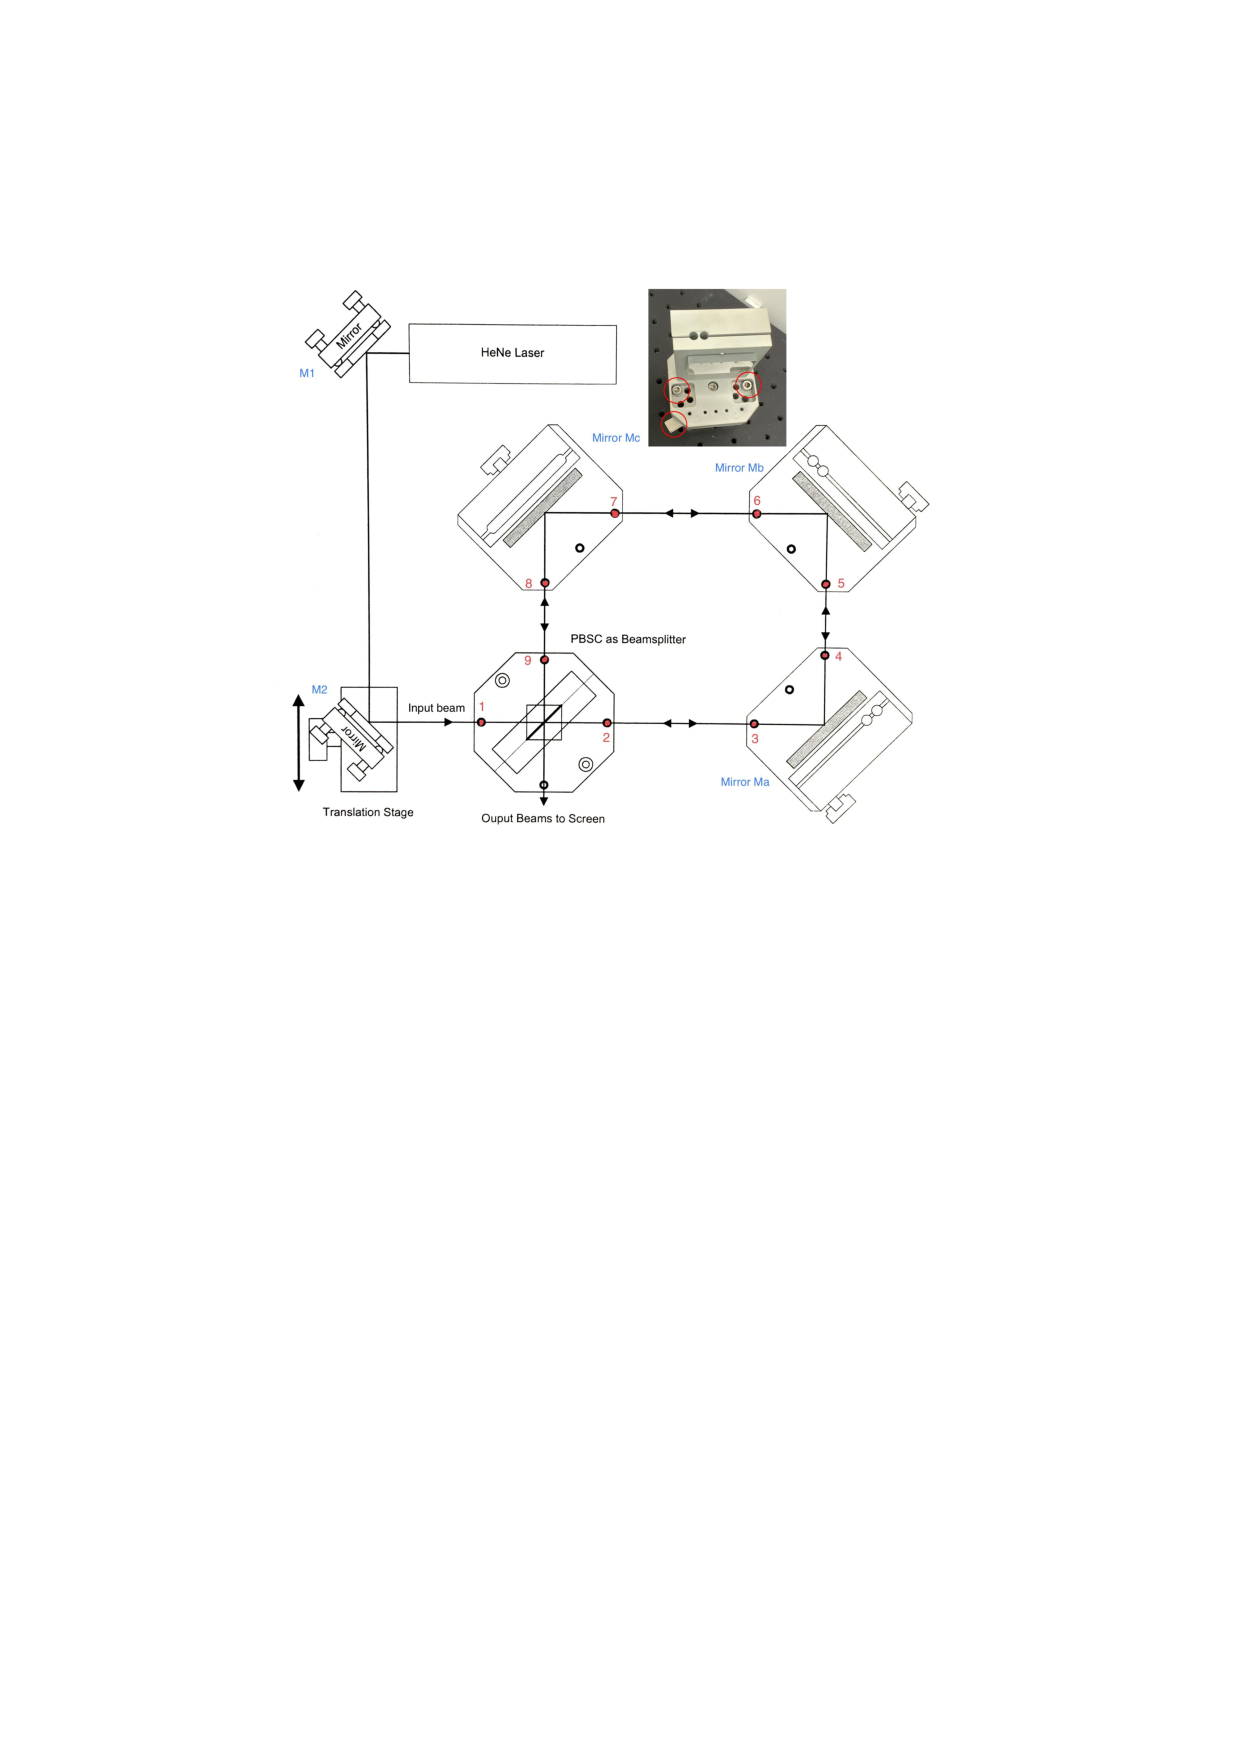
\includegraphics[width = .55\textwidth]{"content/pics/setup.png"}
    \caption{Experimental setup of the measurement of the heat capacity of copper \cite{V47}.}
    \label{fig:setup}
\end{figure}

\subsection{Measurement process}
First, the recipient is evacuated and filled with helium. Liquid nitrogen is poured into the Dewar container to cool the recipient. When a temperature of $\qty{80}{\kelvin}$
(i.e. $R = \qty{22.6}{\milli\ohm}$) is reached, the vacuum pump is turned on to keep the experiment at a constant low pressure. The whole cooling process can take up to an hour.
Now the apparatus is heated using the heating coils. The inner coil should be set to a current of approx. $\qty{160}{\milli\ampere}$ while the outer coil has
to be repeatedly adjusted to match the temperature of the inner coil. In steps of $\qtyrange{7}{11}{\celsius}$ the time interval, the sample temperature (resistance),
as well as the current and voltage of the heating coil are noted. As a reference table \ref{fig:R_T} can be used to determine the resistances corresponding to the desired temperature
intervals.

\begin{figure}
    \centering
    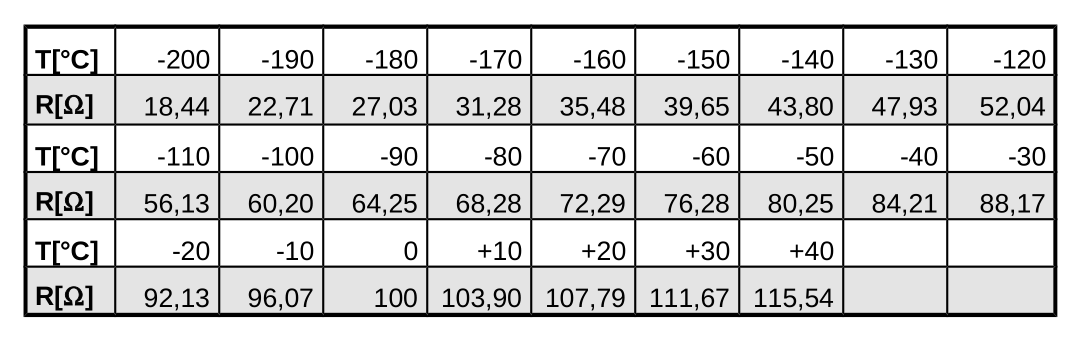
\includegraphics[width = .8\textwidth]{"content/pics/R_T.png"}
    \caption{Resistor values and corresponding temperatures \cite{V47}.}
    \label{fig:R_T}
\end{figure}

The recorded data can be used to calculate the heat capacity at constant pressure $C_{\symup{p}}$ of copper.
